\section{MGGeometry Classes}

 The following is a list of classes in the MGGeometry framework and
a description of their uses.


MGGeometryDetectorConstruction
 
\begin{lstlisting}
    This class is the primary class that builds the MG materials as
    well as instantiates any detector chosen in the
    /MG/geometry/detector messenger described above. It creates a
    world volume and places the detector as a single object inside
    it. Eventually it will first place a shield inside the world
    volume, and then a detector inside the shield, but for now we
    don't have any shields.
   \end{lstlisting}

MGGeometryDetector

\begin{lstlisting}
    This is the base class for all MGGeometry detector classes.
    When instantiated, it must be called with the serial number of
    the desired detector. It allocates a pointer to the outermost
    detector and sets its name. All other functionality must be built
                                within each individual kind of detector class.
   \end{lstlisting}
MGGeometryDetectorMessenger
 
\begin{lstlisting}
    The object that is used to issue commands to the MGGeometry
    framework.
   \end{lstlisting}
MJGeometry800gCrystal MJGeometryCloverDetector MJGeometryCloverInNaIBarrel MJGeometrySolidBlock
 
\begin{lstlisting}
    These are subclasses of the MGGeometryDetector class. These
    classes may contain active detector subparts (e.g.,
    the MJGeometryCloverDetector), but as far as the simulation is
    concerned, these classes correspond to the ``entire'' detector
    detector. (``Entire'' is in quotes because what makes up the
    ``entire'' detector is somewhat subjective. A dewar, for instance,
    may or may not be thought of as part of the detector.)
   \end{lstlisting}
    MJGeometryCloverCrystal
   MJGeometryNaIBarrel
 
\begin{lstlisting}
    These classes are subparts of detectors. For examples, the
    MJGeometryCloverDetector contains pointers to four
    MJGeometryCloverCrystals, and each crystal is treated as a
    separate object. When the four crystals are instantiated as
    part of the MJGeometryCloverDetector, however, the entire
    clover detector is handled as as object incorporating the
    crystals.
   \end{lstlisting}
  

\section{GERDA Geometry}

The GERDA geometry can be chosen by setting the command
 
\begin{lstlisting}
   /MG/geometry/detector [detector]
                    \end{lstlisting}
 in the corresponding macro. For the
standard GERDA geometry, the detector has to be ``GerdaArray". Also
other geometries exist that are related to the GERDA experiment,
i.e. they are either modified geometries or teststands.


The geometry is organized in a group of classes: the following figure gives an
overview of the structure.  
\begin{figure}
\begin{center}
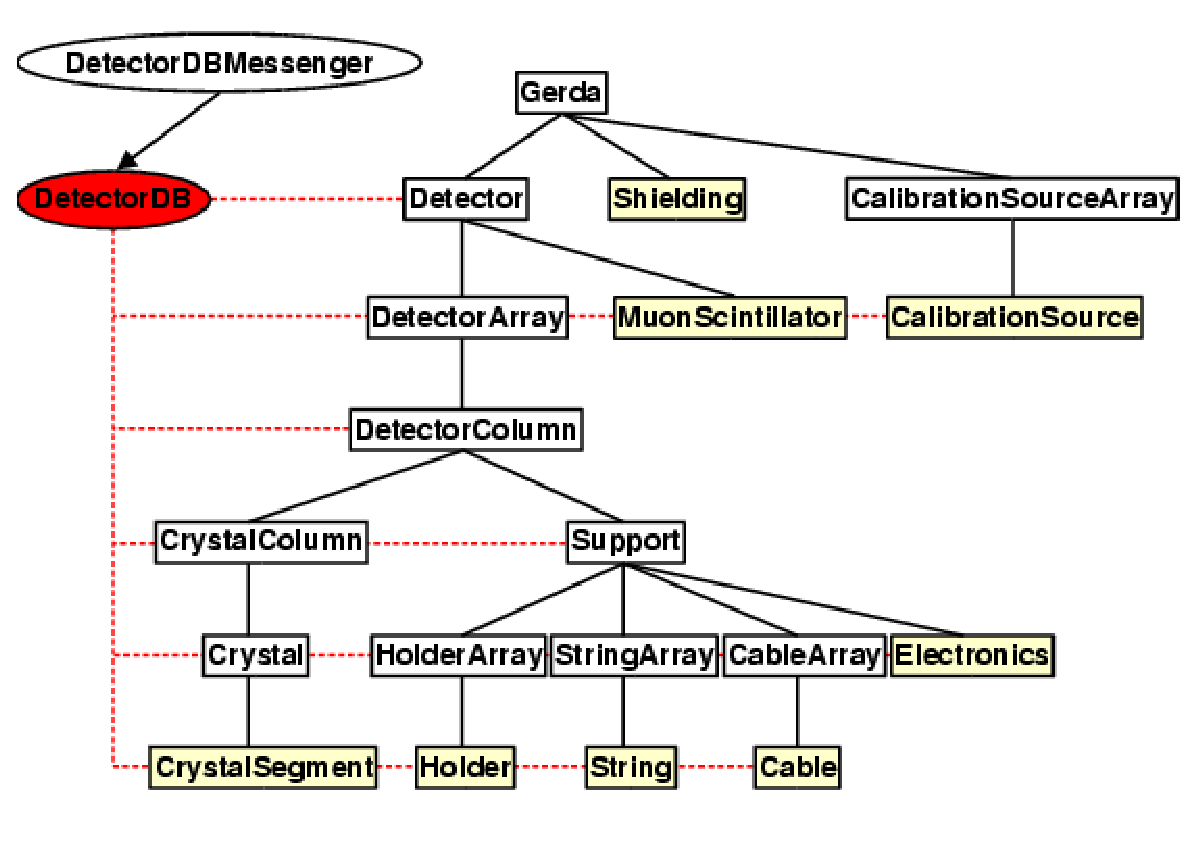
\includegraphics[width=.8\textwidth]{geometryclasses}
\end{center}
\caption{Class structure for GerdaArray}
\end{figure}
The class names in the figure do not
include the prefix GEGeometry since it is common to all classes
displayed. The class ``GEGeometryGerda" inherits from
``MGGeometryDetector", i.e. it is the basic class which gets
instantiated from the MaGe framework. Since the real geometry of the
experiment is still under investigation and not fixed yet, the Monte
Carlo is kept as flexible as possible. For that reason a database
class, ``GEGeometryDetectorDB" is introduced which governs all the
parameters for the geometry. Those parameters can be adjusted by
commands, i.e. there exists a messenger class which controls the
database. As can be seen in the diagram, the database is connected to
all classes in the geometry structure.


The first three branches ``Detector", ``Shielding" and
"CalibrationSourceArray" are rough groupings. In order to focus on
particular parts of the geometry each of those branches can be 
switched off. The calibration sources for example are not needed for 
the study of internal background of the crystals and the support.
The detector itself consists of an array of crystals which is made out
of bare crystals (or crystal segments) and a support structure that
includes holders, strings, cables and electronics. This allows easy
replacements of parts of the geometry for test reasons or changes in
the setup.  Auxiliary detectors are also installed, namely the muon
plastic scintillator on top of the vessel and photomultipliers inside
the water tank (not yet in the Monte Carlo).
The shaded classes are those in which physical volumes are
created. Also, most of the calculations for positioning and
orientation are done via class functions.
In order to add new elements to the simulation new classes are added.
Existing examples are the scintillator and the germanium
detectors. The solids and logical volumes should be introduced in the
database class whereas the physical volume should be instanciated in
the corresponding class. All used parameters are held flexible by
adding the corresponding commands to the database messenger
class. This has to include a flag that controls if the new element is
to be included in the run or not. By following these instructions, the
changes can be submitted to the CVS repository and are made available
for other users


 The following setups are currently available. They are defined by the
settings in the corresponding macros, i.e. the deviation from the
default values of the geometry parameters.
 Phase I:           Unsegmented crystals. So far, this setup is only used in the study of cosmic muons.
 Phase II:          7 strings with 3 crystals. Each crystal is segmented into 6 phi-{} and 3 z-{}segments (standard).
 Simple Test Stand: A standard crystal within an aluminum cryostat which is placed in front of a capsulated
       source and lead bricks. The comparison of Monte Carlo and real data provided a first
       validation of the new MaGe code development.
 
\section{Germanium detectors} 
{\it Kevin} \\ 

\section{Muon veto}
\begin{table}[ht]
 \caption{Overview over the different photomultiplier distributions for the Cherenkov veto for GERDA. \label{Table:pmt_dist}}
 \begin{center}
  \begin{tabular}{|c|c|c|l|}
   \hline
   distributionnumber  & \# of pmts in pillbox & \# of pmts in water & comment \\ \hline \hline
   0                   &                     6 &                  66 & standard distribution \\ \hline
   1                   &                     4 & 70                  & alternative distribution \\ \hline
   -1                  &                     0 &                   0 & no Cherenkov veto \\ \hline
  \end{tabular}
 \end{center}
\end{table}
The GERDA muon veto consists out of two systems. The plastic scintillator panels on top of the penthouse 
and the Cherenkov veto in the water tank surrounding the cryostat. In \mage the plastic panels are hard
coded in the geometry structure, while the Cherenkov veto has some commands to activate it or to select a
different placement of the photomultipliers in the water tank. \\
The photomultipliers in the GERDA geometry are currently constructed out of stainless steel housings and a PET-foil 
covering the upper part of the PMTs. If a photon hits the PET foil, a hit is scored and written into the output file. 
To account for the efficiency of the photomultiplier, it is recommendened to kill four of five photons in the MGManagmentStackingAction.cc, to save simulation time. Otherwise the efficiency has to be considered in the analysis 
of the root files. \\
Currently there are two different distributions, the user can select (see table \ref{Table:pmt_dist}), or one
can simply deactivate the Cherenkvo veto. 

The Cherenkov veto is initiated with the macro command:
\begin{lstlisting}
/MG/geometry/cherenkov distributionnumber
\end{lstlisting}
Of course, the optical processes have to be activated with
\begin{lstlisting}
/MG/processes/optical true
\end{lstlisting}
and the optical output has to be selected:
\begin{lstlisting}
/MG/eventaction/rootschema GerdaArrayOptical
\end{lstlisting}
Otherwise no Cherenkov effect takes part, and no photons are registered with the photomultipliers.
The data is than accumulated in the root output file in the branches \textit{ph\_$\star$} and 
\textit{PMT\_$\star$} for the Cherenkov veto and in the branch \textit{$\star$\_\ scint \_$\star$} for
the plastic panels.


\section{Electronics and calibration sources} 
{\it Daniel} \\ 

\section{Infrastructure} 
{\it Jens} \\ 
